% !TEX root = ../main.tex
\chapter{Monte Carlo Methods}

\textit{Monte Carlo (MC) Methods} are simple and effective approaches to deal with `full' RL problems (without knowing $\mathcal{P}$ and $\mathcal{R}$). These methods only require experience (sample sequences of states, actions and rewards, i.e., real-world data gathered by interacting with the environment) and episodic tasks. MC is our first \textit{model-free} approach, for both prediction and control.

MC methods estimate expectations by averaging over a large number of random samples. 
Since $v_\pi(s)=\mathbb{E}_\pi[G_t\mid S_t=s]$ and $q_\pi(s,a)=\mathbb{E}_\pi[G_t\mid S_t=s,A_t=a]$ are expectations, we can approximate the true expected returns (state-value and action-value functions) with the average of the returns seen if we collect enough data.

Pay attention! Even if $\mathcal{P}$ and $\mathcal{R}$ are not known, we will not use data to estimate such quantities.
For efficiency, we will resort to \textit{model-free} RL approaches, that will estimate instead $\mathrm{v}$ and $\mathrm{q}$ (later directly $\pi$). There are also \textit{model-based} RL approaches.
\section{Prediction: First-visit MC prediction}
We generate an episode and, going backwards, we update the estimate of each visited state with the return observed after its \emph{first} visit: if $S_t$ already appears at an earlier step of the episode, the update is skipped. Only visited states are updated.

\begin{algobox}{First-visit MC prediction, for estimating $V \approx \mathrm{v}_\pi$}
\raggedright
Input: a policy $\pi$ to be evaluated

\medskip
Initialize:\\
\hspace*{1.5em}$V(s) \in \mathbb{R}$, arbitrarily, for all $s \in \mathcal{S}$\\
\hspace*{1.5em}$\mathit{Returns}(s) \leftarrow$ an empty list, for all $s \in \mathcal{S}$

\medskip
Loop forever (for each episode):\\
\hspace*{1.5em}Generate an episode following $\pi$:\\
\hspace*{3em}$S_0, A_0, R_1, S_1, A_1, R_2, \dots, S_{T-1}, A_{T-1}, R_T$\\
\hspace*{1.5em}$G \leftarrow 0$\\
\hspace*{1.5em}Loop for each step of episode, $t = T-1, T-2, \dots, 0$:\\
\hspace*{3em}$G \leftarrow \gamma G + R_{t+1}$\\
\hspace*{3em}Unless $S_t$ appears in $S_0, S_1, \dots, S_{t-1}$:\\
\hspace*{4.5em}Append $G$ to $\mathit{Returns}(S_t)$\\
\hspace*{4.5em}$V(S_t) \leftarrow \operatorname{average}\bigl(\mathit{Returns}(S_t)\bigr)$
\end{algobox}

The \textit{Every-visit} MC prediction algorithm is similar to the first-visit one, but it updates the value of a state every time it appears in an episode, not just the first time. This means that the same state can be updated multiple times in a single episode. So the difference in the pseudo-code is that the \textit{Unless} condition no longer appears. Instead of storing all the returns, a more efficient implementation uses incremental updates:
\[N(S_t)\leftarrow N(S_t)+1,\qquad V(S_t)\leftarrow V(S_t)+\frac{1}{N(S_t)}\bigl[G_t-V(S_t)\bigr]\]
or, with a constant step-size (better for non-stationary problems), $V(S_t)\leftarrow V(S_t)+\alpha\bigl[G_t-V(S_t)\bigr]$.

Some properties of MC prediction:
\begin{itemize}
    \item MC learns directly from experience: there is no need to keep a model of the environment;
    \item the estimate of each state is independent of the estimates of the other states (MC does not bootstrap, unlike DP);
    \item the computation needed to update each state does not depend on the size of the MDP, but on the length of the episode.
\end{itemize}

The reason why we compute the return of each visited state by going backwards from the final time-step is that it requires fewer computations:

\begin{figure}[H]
\centering
\begin{tikzpicture}[>={Stealth[length=2mm]}, font=\small,
    st/.style={circle, draw, minimum size=5mm, inner sep=0pt},
    term/.style={rectangle, draw, fill=gray!50, minimum size=5mm, inner sep=0pt},
    eq/.style={font=\footnotesize},
    cnt/.style={draw, font=\footnotesize, inner sep=3pt}]

  % chain of states with rewards
  \foreach \i in {0,...,4} { \node[st] (s\i) at (1.5*\i, 0) {}; }
  \node[term] (T) at (7.5, 0) {};
  \foreach \i/\j/\r in {0/1/3, 1/2/4, 2/3/7, 3/4/1} {
    \draw[->, thick] (s\i) -- node[above] {\r} (s\j);
  }
  \draw[->, thick] (s4) -- node[above] {2} (T);
  \node[right=8mm of T] {$\gamma = 0.5$};

  % left: backward recursion (staircase)
  \node[eq, anchor=west] at (0.0, -1.3) {$G_0 = R_1 + \gamma G_1$};
  \node[eq, anchor=west] at (0.6, -2.0) {$G_1 = R_2 + \gamma G_2$};
  \node[eq, anchor=west] at (1.2, -2.7) {$G_2 = R_3 + \gamma G_3$};
  \node[eq, anchor=west] at (1.8, -3.4) {$G_3 = R_4 + \gamma G_4$};
  \node[eq, anchor=west] at (2.4, -4.1) {$G_4 = R_5 + \gamma G_5$};
  \node[eq, anchor=west] at (3.0, -4.8) {$G_5 = 0$};
  \node[cnt] at (2.6, -5.7) {5 additions};

  % right: direct sums, right-aligned
  \node[eq, anchor=east] at (12.3, -1.3) {$G_0 = R_1 + \gamma R_2 + \gamma^2 R_3 + \gamma^3 R_4 + \gamma^4 R_5 = 7$};
  \node[eq, anchor=east] at (12.3, -2.0) {$G_1 = R_2 + \gamma R_3 + \gamma^2 R_4 + \gamma^3 R_5 = 8$};
  \node[eq, anchor=east] at (12.3, -2.7) {$G_2 = R_3 + \gamma R_4 + \gamma^2 R_5 = 8$};
  \node[eq, anchor=east] at (12.3, -3.4) {$G_3 = R_4 + \gamma R_5 = 2$};
  \node[eq, anchor=east] at (12.3, -4.1) {$G_4 = R_5 = 2$};
  \node[eq, anchor=east] at (12.3, -4.8) {$G_5 = 0$};
  \node[cnt] at (9.8, -5.7) {10 additions};
\end{tikzpicture}
\caption{Computing the returns of an episode backwards, with
$G_t = R_{t+1} + \gamma G_{t+1}$ (left), reuses the value of $G_{t+1}$ and
needs 5 additions. Evaluating each return as a sum of discounted rewards
(right) needs 10. This is why Monte Carlo methods scan the episode
backwards.}
\label{fig:return-backward}
\end{figure}

\section{Control: Model-free Generalized Policy Iteration (GPI)}
We would like to apply GPI using MC to evaluate the policy, but greedy policy improvement over $V(s)$ (as in dynamic programming) requires a model of the MDP:
\[\pi'(s)=\argmax_{a\in\mathcal{A}}\left(\mathcal{R}_s^a+\gamma\sum_{s'\in\mathcal{S}}\mathcal{P}_{ss'}^aV(s')\right)\]
and now $\mathcal{P}$ and $\mathcal{R}$ are not known.

The solution is to use greedy policy improvement over $Q(s,a)$, which is model-free:
\[\pi'(s)=\argmax_{a\in\mathcal{A}}Q(s,a)\]
In this case we have the (state,action) space that is larger than the state space and we may have several (state, action) pairs unexplored. In MC methods we need to collect data for each (state, action) pair to ensure reaching optimality, and this is not guaranteed, for example, with deterministic policies. We need to adopt strategies that guarantee a certain level of exploration.

\subsection{Control: Exploring Starts (ES)}
A simple strategy to ensure exploration is ES. With this method we ensure that episodes start in every state-action pair (each pair has non-zero probability of being selected as the start), and then the agent follows the current policy. 
\begin{algobox}{Monte Carlo ES (Exploring Starts), for estimating $\pi \approx \pi_*$}
\raggedright
Initialize:\\
\hspace*{1.5em}$\pi(s) \in \mathcal{A}(s)$ (arbitrarily), for all $s \in \mathcal{S}$\\
\hspace*{1.5em}$Q(s,a) \in \mathbb{R}$ (arbitrarily), for all $s \in \mathcal{S},\, a \in \mathcal{A}(s)$\\
\hspace*{1.5em}$\mathit{Returns}(s,a) \leftarrow$ an empty list, for all $s \in \mathcal{S},\, a \in \mathcal{A}(s)$

\medskip
Loop forever (for each episode):\\
\hspace*{1.5em}Choose $S_0 \in \mathcal{S},\, A_0 \in \mathcal{A}(S_0)$ randomly such that all pairs have probability $> 0$\\
\hspace*{1.5em}Generate an episode from $S_0, A_0$, following $\pi$:\\
\hspace*{3em}$S_0, A_0, R_1, \dots, S_{T-1}, A_{T-1}, R_T$\\
\hspace*{1.5em}$G \leftarrow 0$\\
\hspace*{1.5em}Loop for each step of episode, $t = T-1, T-2, \dots, 0$:\\
\hspace*{3em}$G \leftarrow \gamma G + R_{t+1}$\\
\hspace*{3em}Unless the pair $S_t, A_t$ appears in $S_0, A_0, S_1, A_1, \dots, S_{t-1}, A_{t-1}$:\\
\hspace*{4.5em}Append $G$ to $\mathit{Returns}(S_t,A_t)$\\
\hspace*{4.5em}$Q(S_t,A_t) \leftarrow \operatorname{average}\bigl(\mathit{Returns}(S_t,A_t)\bigr)$\\
\hspace*{4.5em}$\pi(S_t) \leftarrow \arg\max_a Q(S_t,a)$
\end{algobox}

For two consecutive policies ($\pi_k$ and $\pi_{k+1}$):
\begin{equation}
  \begin{split}
    q_{\pi_k}(s,\pi_{k+1}(s))&=q_{\pi_k}(s,\arg\max_a q_{\pi_k}(s,a))\\
    &=\max_a q_{\pi_k}(s,a)\\
    &\geq q_{\pi_k}(s,\pi_k(s))=v_{\pi_k}(s)
  \end{split}
\end{equation}
For all states, the next policy is better than or equal to the previous one (assuming exact action values). In practice MC ES works, but its convergence to the optimal policy has not been formally proved.

However, in many scenarios, it is impossible to start an episode with all the possible (state,action) pairs. For this reason we look at different approaches to ensure exploration without ES.
\subsection{Control: \texorpdfstring{$\epsilon$}{epsilon}-greedy and \texorpdfstring{$\epsilon$}{epsilon}-soft policies}
We can resort to stochastic policies like the $\varepsilon$-greedy policy seen for bandits:
\[
A_t \overset{\mathrm{def}}{=}
\begin{cases}
\text{greedy action} & \text{with probability } 1-\varepsilon,\\
\text{a random action (among all actions)} & \text{with probability } \varepsilon.
\end{cases}
\]
More generally, we can resort to \textit{soft policies}, i.e., stochastic policies that have $\pi(a|s)>0$ for all $a$ and $s$.

We call \textit{$\varepsilon$-soft policies} the soft policies that have $\pi(a|s)\geq\frac{\varepsilon}{|\mathcal{A}(s)|}$ for all $a$ and $s$, for some $\varepsilon>0$ ($\varepsilon$-greedy is the greediest $\varepsilon$-soft policy). $\varepsilon$ governs the trade-off between exploration and exploitation.

\begin{figure}[htbp]
\centering
\begin{tikzpicture}[
    x=0.85cm,
    y=0.85cm,
    bar/.style={draw=black, thick, fill=cyan!30},
    title/.style={font=\bfseries\large},
    axislabel/.style={font=\bfseries}
]

% ---------- EPSILON-GREEDY ----------
\node[title] at (2.5,5.5) {$\varepsilon$-Greedy policies};

% Plot frame
\draw[gray] (0,0) rectangle (5,4);

% Bars
\foreach \x in {0.25,1.0,1.75,2.5,4.0} {
    \draw[bar] (\x,0) rectangle ++(0.55,0.15);
}
\draw[bar] (3.25,0) rectangle ++(0.55,3.2);

% Labels
\node[axislabel, anchor=east] at (-0.05,2)
    {Probability};
\node[axislabel] at (2.5,-0.5) {Action};
\node[
    font=\bfseries\small,
    text=red!50!black
] at (3.4,3.55) {Greedy action};

% ---------- SET INCLUSION ----------
\node[
    font=\Huge,
    text=red!55!black
] at (6.4,5.4) {$\subset$};

% ---------- EPSILON-SOFT ----------
\begin{scope}[xshift=7cm]

\node[title] at (2.5,5.5) {$\varepsilon$-Soft policies};

% Plot frame
\draw[gray] (0,0) rectangle (5,4);

% Bars
\draw[bar] (0.25,0) rectangle ++(0.55,0.45);
\draw[bar] (1.0,0) rectangle ++(0.55,1.65);
\draw[bar] (1.75,0) rectangle ++(0.55,0.5);
\draw[bar] (2.5,0) rectangle ++(0.55,0.45);
\draw[bar] (3.25,0) rectangle ++(0.55,0.35);
\draw[bar] (4.0,0) rectangle ++(0.55,0.55);

% Labels
\node[axislabel, anchor=east] at (-0.05,2)
    {Probability};
\node[axislabel] at (2.5,-0.5) {Action};

% Epsilon-soft lower bound
\draw[
    red!55!black,
    dashed,
    thick
] (-0.3,0.12) -- (5.3,0.12);

\node[
    text=red!55!black,
    font=\large,
    anchor=east
] at (-0.55,0.12)
    {$\dfrac{\varepsilon}{|\mathcal{A}|}$};

\end{scope}

\end{tikzpicture}
\end{figure}


\begin{algobox}{On-policy first-visit MC control (for $\varepsilon$-soft policies), for estimating $\pi \approx \pi_*$}
\raggedright
Algorithm parameter: small $\varepsilon > 0$

\medskip
Initialize:\\
\hspace*{1.5em}$\pi \leftarrow$ an arbitrary $\varepsilon$-soft policy\\
\hspace*{1.5em}$Q(s,a) \in \mathbb{R}$ (arbitrarily), for all $s \in \mathcal{S},\, a \in \mathcal{A}(s)$\\
\hspace*{1.5em}$\mathit{Returns}(s,a) \leftarrow$ an empty list, for all $s \in \mathcal{S},\, a \in \mathcal{A}(s)$

\medskip
Repeat forever (for each episode):\\
\hspace*{1.5em}Generate an episode following $\pi$:\\
\hspace*{3em}$S_0, A_0, R_1, \dots, S_{T-1}, A_{T-1}, R_T$\\
\hspace*{1.5em}$G \leftarrow 0$\\
\hspace*{1.5em}Loop for each step of episode, $t = T-1, T-2, \dots, 0$:\\
\hspace*{3em}$G \leftarrow \gamma G + R_{t+1}$\\
\hspace*{3em}Unless the pair $S_t,A_t$ appears in $S_0,A_0,S_1,A_1,\dots,S_{t-1},A_{t-1}$:\\
\hspace*{4.5em}Append $G$ to $\mathit{Returns}(S_t,A_t)$\\
\hspace*{4.5em}$Q(S_t,A_t) \leftarrow \operatorname{average}\bigl(\mathit{Returns}(S_t,A_t)\bigr)$\\
\hspace*{4.5em}$A^* \leftarrow \arg\max_a Q(S_t,a)$ (with ties broken arbitrarily)\\
\hspace*{4.5em}For all $a \in \mathcal{A}(S_t)$:
\[
\hspace*{6em}
\pi(a \mid S_t) \leftarrow
\begin{cases}
1-\varepsilon+\dfrac{\varepsilon}{|\mathcal{A}(S_t)|}
& \text{if } a=A^*,\\[6pt]
\dfrac{\varepsilon}{|\mathcal{A}(S_t)|}
& \text{if } a\neq A^*.
\end{cases}
\]
\end{algobox}

It can be shown (policy improvement theorem) that the previous algorithm allows improvement, but $\varepsilon$-soft policies are not optimal. However they may work quite well and may represent a feasible option when ES cannot be applied. 

\subsection{Prediction/Control: On-policy vs Off-policy learning}
What we have seen so far is \textit{on-policy} learning (`learning on the job'), i.e., the agent learns about the policy it is following. \textit{Off-policy} learning (`looking over someone's shoulder') is learning about policy $\pi$ (target policy) from experience sampled from policy $b$ (behaviour policy). The behavior policy is the one that generates the data, while the target policy is the one that we want to learn about.
Why using a behaviour policy?
\begin{itemize}
  \item we can leave the exploration to the behaviour policy and reach optimal policies;
  \item we can gain experience by observing other agents (or humans);
  \item we can re-use experience generated from old policies $\pi_1,\pi_2,\dots,\pi_{k-1}$;
  \item we can learn multiple policies while following one policy.
\end{itemize}
If we resort to off-policy learning we must ensure:
\begin{enumerate}
  \item Knowledge of $b(a|s)$ (and of the target policy);
  \item Coverage: $\pi(a|s)>0 \implies b(a|s)>0$.
\end{enumerate}
Coverage means that the behaviour policy must explore the (state, action) pairs that have non-zero probability under the target policy: if this does not happen, the agent cannot learn the correct action value for that state since it never observed samples of what would happen.

Almost all off-policy methods use \textit{importance sampling}, a technique for estimating expected values under one distribution given samples from another.
In off-policy we have: 
\[
\mathbb{E}_{\pi}[X]
= \sum_{x \in \mathcal{X}} x\pi(x)
= \sum_{x \in \mathcal{X}} x\pi(x)\frac{b(x)}{b(x)}
= \sum_{x \in \mathcal{X}} x\rho(x)b(x)
= \mathbb{E}_{b}[X\rho(X)]
\]
where $\rho(x)=\frac{\pi(x)}{b(x)}$ is called the \textit{importance sampling ratio} and the samples are drawn as $x\sim b$. We can consider $X\rho(X)$ as a new random variable.
To actually use this with data, we use Monte Carlo to approximate this expectation by computing the average of the weighted samples:
\[
\mathbb{E}_{\pi}[X] \approx \frac{1}{n} \sum_{i=1}^{n} x_i \rho(x_i)
\]
\begin{esempio}{Importance sampling in a 2-armed bandit}
The target policy $\pi$ chooses $a_1$ with probability 0.75 and $a_2$ with probability 0.25; we observe another agent with behaviour policy $b$ that chooses each action with probability 0.5. Initial estimates are $q_b(a_i)=q_\pi(a_i)=0$.
\begin{itemize}
    \item Episode 1: $a_2\to+1$, so $q_b(a_2)=1$ and $q_\pi(a_2)=1\cdot\frac{0.25}{0.5}=0.5$;
    \item Episode 2: $a_1\to-1$, so $q_b(a_1)=-1$ and $q_\pi(a_1)=-1\cdot\frac{0.75}{0.5}=-1.5$;
    \item Episode 3: $a_1\to+2$, so $q_b(a_1)=\frac{-1+2}{2}=0.5$ and $q_\pi(a_1)=0.5\cdot\frac{0.75}{0.5}=0.75$.
\end{itemize}
\end{esempio}

In RL we have to deal with sequences: we use returns generated by $b$ to evaluate $\pi$, so we cannot compute $v_\pi$ directly as the average of the returns seen. We have to correct each return with importance sampling.
Given a starting state $S_t$, the probability of the subsequent state-action trajectory under policy $\pi$ is:
\begin{equation}
  \begin{split}
    &\Pr\left\{A_t,S_{t+1},A_{t+1},\dots,S_T\mid S_t,A_{t:T-1}\sim\pi\right\}\\
    &=\pi(A_t|S_t)p(S_{t+1}|S_t,A_t)\pi(A_{t+1}|S_{t+1})\cdots p(S_T|S_{T-1},A_{T-1})\\
    &=\prod_{k=t}^{T-1} \pi(A_k|S_k)p(S_{k+1}|S_k,A_k)
  \end{split}
\end{equation}
We can compute the relative probability of the trajectory under the target and the behaviour policy (the importance-sampling ratio) as follows:
\[
\rho_{t:T-1}
\doteq
\frac{
\prod_{k=t}^{T-1} \pi(A_k \mid S_k)\,p(S_{k+1} \mid S_k,A_k)
}{
\prod_{k=t}^{T-1} b(A_k \mid S_k)\,p(S_{k+1} \mid S_k,A_k)
}
=
\prod_{k=t}^{T-1}
\frac{\pi(A_k \mid S_k)}{b(A_k \mid S_k)}
\]
The transition probabilities cancel out, so the ratio only depends on the two policies. We can now exploit the returns obtained with $b$ to estimate $v_\pi$ with Monte Carlo:
\[\mathbb{E}_b[\rho_{t:T-1}G_t\mid S_t=s]=v_\pi(s)\]
We can consider the importance sampling ratios as weights. 

\begin{algobox}{Off-policy MC prediction (Every-Visit, weighted IS), for estimating $Q \approx q_\pi$}
\raggedright
Input: an arbitrary target policy $\pi$

\medskip
Initialize, for all $s \in \mathcal{S},\, a \in \mathcal{A}(s)$:\\
\hspace*{1.5em}$Q(s,a) \in \mathbb{R}$ (arbitrarily)\\
\hspace*{1.5em}$C(s,a) \leftarrow 0$

\medskip
Loop forever (for each episode):\\
\hspace*{1.5em}$b \leftarrow$ any policy with coverage of $\pi$\\
\hspace*{1.5em}Generate an episode following $b$:\\
\hspace*{3em}$S_0, A_0, R_1, \dots, S_{T-1}, A_{T-1}, R_T$\\
\hspace*{1.5em}$G \leftarrow 0$\\
\hspace*{1.5em}$W \leftarrow 1$\\
\hspace*{1.5em}Loop for each step of episode, $t = T-1, T-2, \dots, 0$, while $W \neq 0$:\\
\hspace*{3em}$G \leftarrow \gamma G + R_{t+1}$\\
\hspace*{3em}$C(S_t,A_t) \leftarrow C(S_t,A_t) + W$\\
\hspace*{3em}$Q(S_t,A_t) \leftarrow Q(S_t,A_t) +
\dfrac{W}{C(S_t,A_t)}
\bigl[G-Q(S_t,A_t)\bigr]$\\
\hspace*{3em}$W \leftarrow W \dfrac{\pi(A_t \mid S_t)}{b(A_t \mid S_t)}$
\end{algobox}


\begin{algobox}{Off-policy MC prediction (Every-Visit, ordinary IS), for estimating $V \approx v_\pi$}
\raggedright
Input: target policy $\pi$, behavior policy $b$, discount $\gamma$\\
Output: estimate $V \approx v_\pi$

\medskip
Initialize:\\
\hspace*{1.5em}$V(s) \in \mathbb{R}$ arbitrarily, for all $s \in \mathcal{S}$, with $V(\text{terminal}) = 0$\\
\hspace*{1.5em}$N(s) \leftarrow 0$, for all $s \in \mathcal{S}$

\medskip
Loop forever (for each episode):\\
\hspace*{1.5em}Generate an episode following $b$:\\
\hspace*{3em}$S_0, A_0, R_1, \dots, S_{T-1}, A_{T-1}, R_T$\\
\hspace*{1.5em}$G \leftarrow 0$, $W \leftarrow 1$\\
\hspace*{1.5em}Loop for each step of episode, $t = T-1, T-2, \dots, 0$, while $W \neq 0$:\\
\hspace*{3em}$G \leftarrow \gamma G + R_{t+1}$\\
\hspace*{3em}$W \leftarrow W \dfrac{\pi(A_t \mid S_t)}{b(A_t \mid S_t)}$\\
\hspace*{3em}$N(S_t) \leftarrow N(S_t) + 1$\\
\hspace*{3em}$V(S_t) \leftarrow V(S_t) +
\dfrac{1}{N(S_t)}\bigl[W \cdot G - V(S_t)\bigr]$
\end{algobox}
The two algorithms differ in both the importance sampling weights and the update rules. When estimating $V(S_t)$, the importance sampling weight must include the probability ratio of the current action $A_t$, since this action is selected according to the behavior policy $b$. In contrast, when estimating $Q(S_t,A_t)$, the current action is already fixed, so only subsequent actions need to be corrected. This explains why $W$ is updated before $V$ but after $Q$.

Moreover, the two algorithms use different importance sampling estimators: $V$ is updated using Ordinary Importance Sampling, which averages the weighted returns using the visit count $N(s)$, whereas $Q$ uses Weighted Importance Sampling, which normalizes the weighted returns by the cumulative weights $C(s,a)$.

Both Ordinary and Weighted Importance Sampling can be used to estimate either $v_\pi(s)$ or $q_\pi(s,a)$. The distinction lies in how the weighted returns are normalized, rather than in the value function being estimated. Both algorithms perform off-policy Monte Carlo prediction (policy evaluation), since they estimate the value of a fixed target policy without improving it.

The slides use the ordinary-IS algorithm for $V$ as a simplified version of the one in the book.

To apply off-policy Monte Carlo control we should keep in mind that coverage can change over time: if $\pi$ is improved to $\pi'$, it is not guaranteed that $\pi'(a|s)>0\implies b(a|s)>0$. In practice off-policy MC control is not effective: over many steps, off-policy estimates have very high variance and are slow to converge. However, \textit{Temporal Difference Learning} will make off-policy learning work in practice.